\documentclass[a4paper,11pt,onecolumn]{IEEEtran}

%% Language and encoding
\usepackage[utf8x]{inputenc}
\usepackage[L7x]{fontenc}
\usepackage[lithuanian]{babel}
\usepackage{graphicx}
\usepackage{epstopdf}
\RequirePackage[skip=5pt,labelfont=bf,justification=centering,labelsep=space]{caption}


\author{Maksim Norkin\\Vilniaus Gedimino technikos universitetas\\Elektronikos fakultetas\\Elektroninių sistemų katedra\\\texttt{maksim.norkin@ieee.org}}
\title{Bakalauro baigiamasis darbas\\Parkinsono ligos eigos stebėjimo priemonė\\2 Plakatas}

\begin{document}

	\maketitle
	
	\begin{figure}[!b]
	\centering
	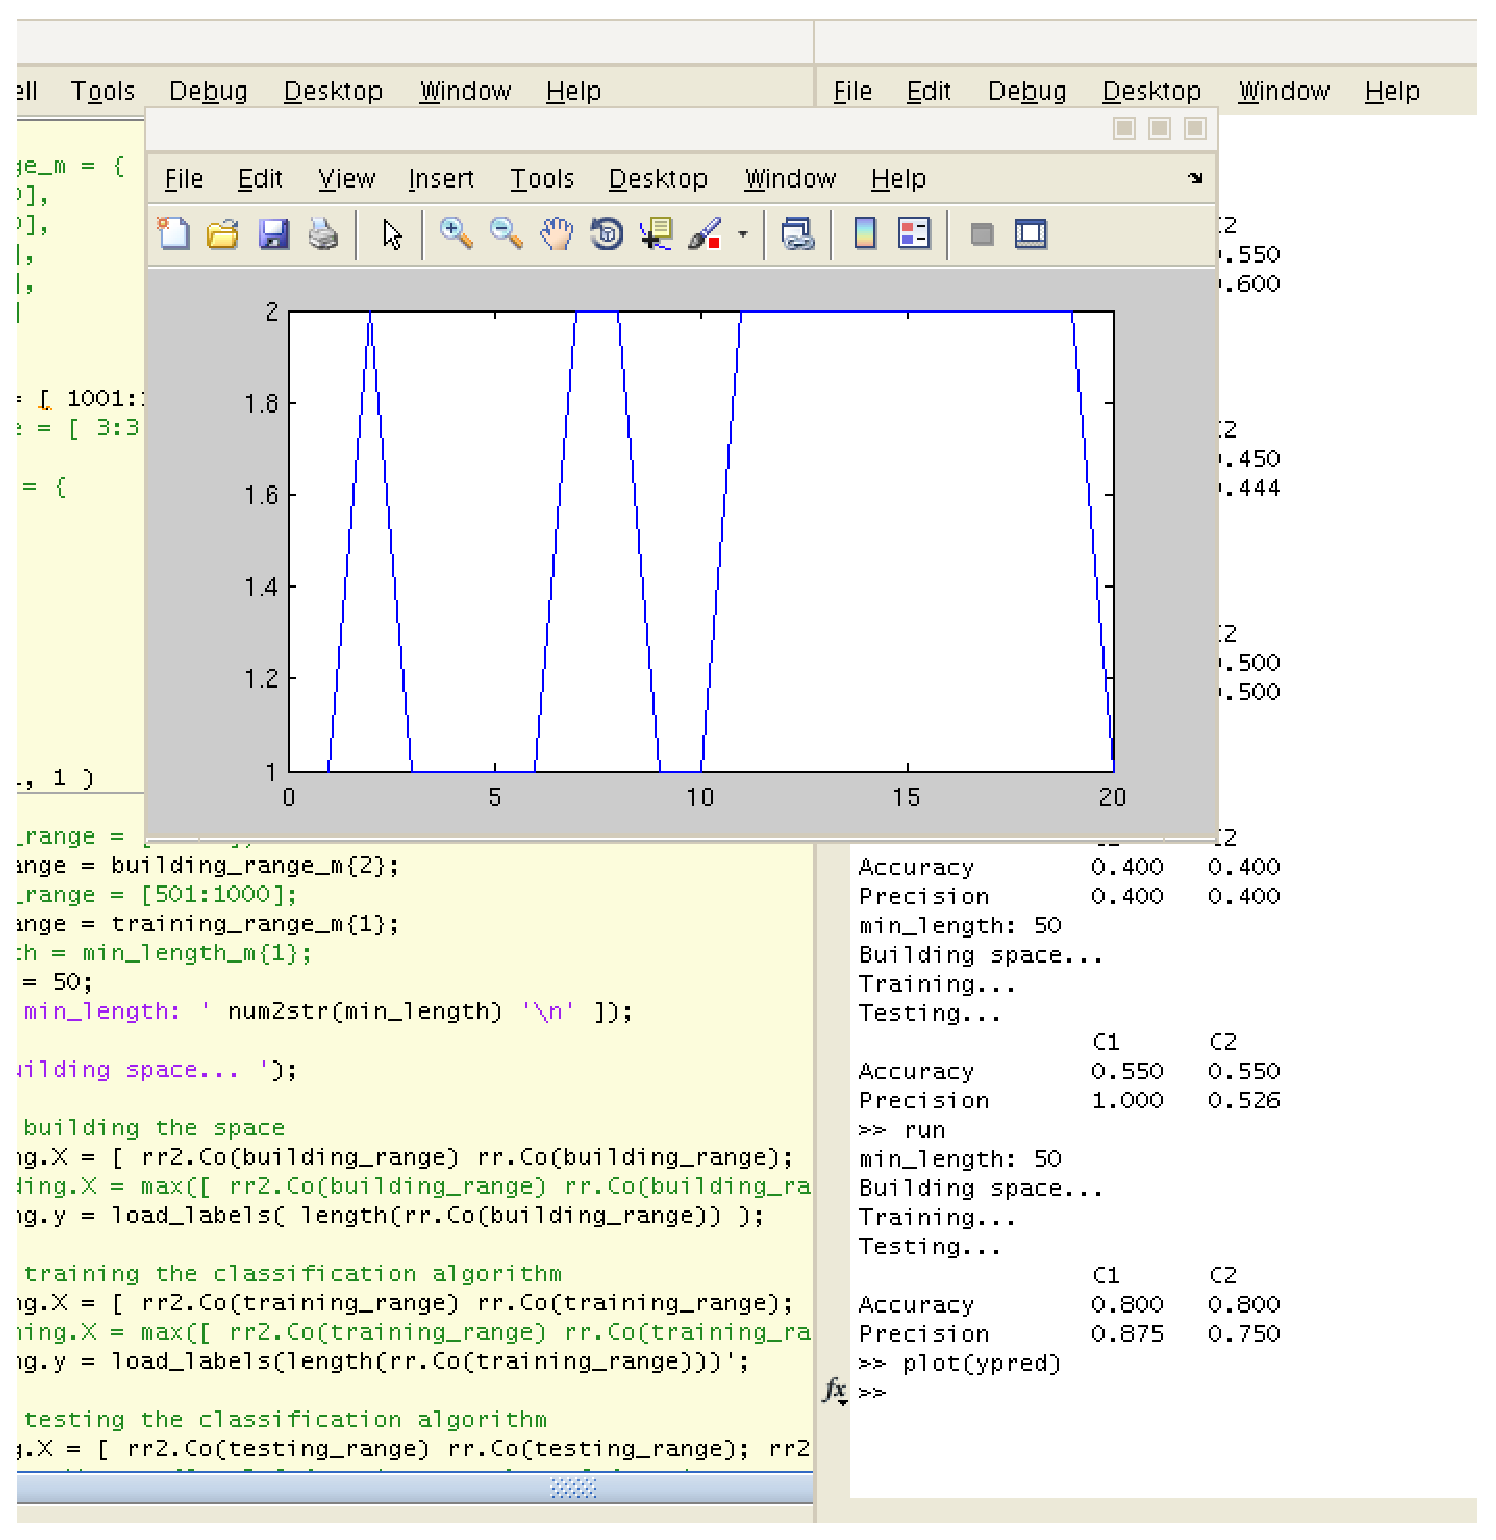
\includegraphics[width=430px]{screen}
	\caption{Programos veikimo rezultato momentinė ekrano kopija}
	\end{figure}


\end{document}